% !TEX root = chapter-standalone.tex

\section{The graphical calculus of string diagrams}\label{sec:graphical-calculus}

% Styles for the string diagrams of this section.
\tikzset{
    sdwire/.style={draw=objects, thick},
    sdbox/.style={block, inner sep=2pt, minimum width=7.5mm, minimum height=6.5mm},
    sdlab/.style={font=\footnotesize, inner sep=1.5pt},
    sdframe/.style={draw=black!50, densely dashed, rounded corners=2pt},
    sdcut/.style={draw=black!60, densely dashed},
}

Throughout this chapter we have been drawing morphisms as boxes with wires attached to them, as in \cref{fig:stacked-morphisms} and \cref{fig:triple-stacked}.
So far, these pictures were illustrations which accompanied the formulas.
In this section explain how a picture of this kind, called a \emph{string diagram}, can be understood as formal mathematics that we can calculate with just as reliably as with formulas, and often much more easily.

Why are pictures a good idea here?
In a strict monoidal category there are two ways of composing morphisms: in series, using $\mthen$, and in parallel, using $\mtimescatmor$.
A morphism which is built using both is a two-dimensional thing: some of its parts come one after the other, and some of them sit side by side.
A formula, however, is a one-dimensional string of symbols.
To squeeze a two-dimensional arrangement into a line we are forced to make choices: where to put the parentheses, where to insert identity morphisms, and which of two independent parts to mention first.
These choices have nothing to do with the morphism that we want to describe, and the conditions in the definition of a strict monoidal category (\cref{def:strict-monoidal-cat}) say precisely that they do not matter.
In a string diagram, these choices are never made in the first place.
As a result, many equations which need a calculation when they are written as formulas are simply \emph{visible} in the pictures.

This way of thinking is very familiar in engineering: block diagrams, signal-flow diagrams, and circuit diagrams all describe a system by drawing its components as boxes and connecting them with wires.
String diagrams make this practice precise, and they work in the same way in every strict monoidal category.

Throughout this section, $\tup{\CatC, \mtimescat, \idmoncat}$ is a strict monoidal category.
We read all diagrams from left to right for series composition, and from top to bottom for parallel composition.

\subsection{Boxes and wires}
\label{sec:string-diagrams-boxes-and-wires}

We start with the dictionary which translates between formulas and pictures.
The basic principle is: \emph{wires stand for objects, and boxes stand for morphisms}.

\paragraph{Morphisms}
A morphism $\mora \colon \Obja \mto \Objb$ is drawn as a box labeled $\mora$, with a wire entering it from the left, labeled by the source $\Obja$, and a wire leaving it to the right, labeled by the target $\Objb$:
\begin{equation}
    \label{eq:string-diagram-morphism}
    \begin{tikzpicture}[baseline=(f.base)]
        \node[sdbox] (f) at (0,0) {$\mora$};
        \draw[sdwire] (f.west) -- ++(-1.3,0) node[sdlab, above, pos=0.6] {$\Obja$};
        \draw[sdwire] (f.east) -- ++(1.3,0) node[sdlab, above, pos=0.6] {$\Objb$};
    \end{tikzpicture}
    \qquad \qquad
    \mora \colon \Obja \mto \Objb
\end{equation}

\paragraph{Series composition}
Given $\mora \colon \Obja \mto \Objb$ and $\morb \colon \Objb \mto \Objc$, their series composition $\mora \mthen \morb$ is drawn by placing the box for $\morb$ to the right of the box for $\mora$, and connecting the output wire of $\mora$ to the input wire of $\morb$:
\begin{equation}
    \label{eq:string-diagram-series}
    \begin{tikzpicture}[baseline=(f.base)]
        \node[sdbox] (f) at (0,0) {$\mora$};
        \node[sdbox] (g) at (2.1,0) {$\morb$};
        \draw[sdwire] (f.west) -- ++(-1.1,0) node[sdlab, above, pos=0.6] {$\Obja$};
        \draw[sdwire] (f.east) -- (g.west) node[sdlab, above, midway] {$\Objb$};
        \draw[sdwire] (g.east) -- ++(1.1,0) node[sdlab, above, pos=0.6] {$\Objc$};
    \end{tikzpicture}
    \qquad \qquad
    \mora \mthen \morb \colon \Obja \mto \Objc
\end{equation}
Two wires can only be connected if they carry the same label.
This is exactly the condition under which two morphisms can be composed in series: the target of the first must be the source of the second.

\paragraph{Parallel composition}
Given $\mora \colon \Obja \mto \Objb$ and $\morb \colon \Objc \mto \Objd$, their parallel composition $\mora \mtimescatmor \morb$ is drawn by placing the box for $\mora$ above the box for $\morb$:
\begin{equation}
    \label{eq:string-diagram-parallel}
    \begin{tikzpicture}[baseline=(current bounding box.center)]
        \node[sdbox] (f) at (0,0.5) {$\mora$};
        \node[sdbox] (g) at (0,-0.5) {$\morb$};
        \draw[sdwire] (f.west) -- ++(-1.3,0) node[sdlab, above, pos=0.6] {$\Obja$};
        \draw[sdwire] (f.east) -- ++(1.3,0) node[sdlab, above, pos=0.6] {$\Objb$};
        \draw[sdwire] (g.west) -- ++(-1.3,0) node[sdlab, above, pos=0.6] {$\Objc$};
        \draw[sdwire] (g.east) -- ++(1.3,0) node[sdlab, above, pos=0.6] {$\Objd$};
    \end{tikzpicture}
    \qquad \qquad
    \mora \mtimescatmor \morb \colon \Obja \mtimescatob \Objc \mto \Objb \mtimescatob \Objd
\end{equation}
Reading the wires on the left from top to bottom gives the source $\Obja \mtimescatob \Objc$, and reading the wires on the right from top to bottom gives the target $\Objb \mtimescatob \Objd$.
In contrast to series composition, no condition is needed: any two boxes can be placed on top of each other.

\paragraph{Identity morphisms}
The identity morphism $\catidat{\Obja}$ is drawn as a wire labeled $\Obja$, without any box:
\begin{equation}
    \label{eq:string-diagram-identity}
    \begin{tikzpicture}[baseline=-0.6ex]
        \draw[sdwire] (0,0) -- (3.3,0) node[sdlab, above, midway] {$\Obja$};
    \end{tikzpicture}
    \qquad \qquad
    \catidat{\Obja} \colon \Obja \mto \Obja
\end{equation}
This fits the intuition: a wire transports whatever it carries from one end to the other, and does nothing to it.

\paragraph{The monoidal unit}
The monoidal unit $\idmoncat$ is not drawn at all: it is ``no wire''.
Accordingly, its identity morphism $\catidat{\idmoncat}$ is the empty picture.
This convention makes it possible to draw boxes which have no input wires, no output wires, or no wires whatsoever:
\begin{equation}
    \label{eq:string-diagram-unit}
    \begin{array}{c@{\qquad\quad}c@{\qquad\quad}c}
        \begin{tikzpicture}[baseline=(s.base)]
            \node[sdbox] (s) at (0,0) {$\mora$};
            \draw[sdwire] (s.east) -- ++(1.1,0) node[sdlab, above, pos=0.6] {$\Obja$};
        \end{tikzpicture}
         &
        \begin{tikzpicture}[baseline=(e.base)]
            \node[sdbox] (e) at (0,0) {$\morb$};
            \draw[sdwire] (e.west) -- ++(-1.1,0) node[sdlab, above, pos=0.6] {$\Obja$};
        \end{tikzpicture}
         &
        \begin{tikzpicture}[baseline=(a.base)]
            \node[sdbox] (a) at (0,0) {$\morc$};
        \end{tikzpicture}
        \\[1.5ex]
        \mora \colon \idmoncat \mto \Obja
         &
        \morb \colon \Obja \mto \idmoncat
         &
        \morc \colon \idmoncat \mto \idmoncat
    \end{array}
\end{equation}
For instance, in $\SetL$ the monoidal unit is the set whose only element is the empty tuple (\cref{lem:SetL-strict-monoidal}), and so a morphism $\idmoncat \mto \Obja$ is the same thing as a choice of one element of $\Obja$.
A box without input wires is thus a way of feeding a fixed value into a diagram.

\paragraph{Boxes with several wires}
A morphism whose source or target is a monoidal product of several objects is drawn as a box with several input or output wires, one for each factor, in the order of the factors from top to bottom:
\begin{equation}
    \label{eq:string-diagram-several-wires}
    \begin{tikzpicture}[baseline=(f.base)]
        \node[sdbox, minimum height=14mm] (f) at (0,0) {$\mora$};
        \draw[sdwire] ([yshift=3mm]f.west) -- ++(-1.3,0) node[sdlab, above, pos=0.6] {$\Obja$};
        \draw[sdwire] ([yshift=-3mm]f.west) -- ++(-1.3,0) node[sdlab, above, pos=0.6] {$\Objb$};
        \draw[sdwire] ([yshift=4.7mm]f.east) -- ++(1.3,0) node[sdlab, above, pos=0.6] {$\Objc$};
        \draw[sdwire] (f.east) -- ++(1.3,0) node[sdlab, above, pos=0.6] {$\Objd$};
        \draw[sdwire] ([yshift=-4.7mm]f.east) -- ++(1.3,0) node[sdlab, above, pos=0.6] {$\Obje$};
    \end{tikzpicture}
    \qquad \qquad
    \mora \colon \Obja \mtimescatob \Objb \mto \Objc \mtimescatob \Objd \mtimescatob \Obje
\end{equation}
Note that we did not write any parentheses in the source and the target of $\mora$.
We do not need to, because the monoidal product of a strict monoidal category is associative on the nose.

\begin{remark}[Conventions]
    There are several conventions for drawing string diagrams.
    We draw series composition from left to right, as is usual for block diagrams in engineering, and as matches our notation $\mora \mthen \morb$.
    In the literature one also finds diagrams which are read from bottom to top, or from top to bottom.
    This is only a matter of rotating the page.
    The word ``string'' refers to the wires; ``wiring diagram'' would be an equally good name.
\end{remark}

\subsection{Why the pictures are unambiguous}
\label{sec:string-diagrams-unambiguous}

A picture is only useful as a notation if it denotes \emph{one} morphism.
At first sight, there is a problem: the pictures of the previous subsection contain less information than the formulas.
Consider three boxes in a row:
\begin{equation}
    \label{eq:string-diagram-three-in-series}
    \begin{tikzpicture}[baseline=(f.base)]
        \node[sdbox] (f) at (0,0) {$\mora$};
        \node[sdbox] (g) at (1.9,0) {$\morb$};
        \node[sdbox] (h) at (3.8,0) {$\morc$};
        \draw[sdwire] (f.west) -- ++(-1.0,0) node[sdlab, above, pos=0.6] {$\Obja$};
        \draw[sdwire] (f.east) -- (g.west) node[sdlab, above, midway] {$\Objb$};
        \draw[sdwire] (g.east) -- (h.west) node[sdlab, above, midway] {$\Objc$};
        \draw[sdwire] (h.east) -- ++(1.0,0) node[sdlab, above, pos=0.6] {$\Objd$};
    \end{tikzpicture}
\end{equation}
Does this picture mean $(\mora \mthen \morb) \mthen \morc$, or does it mean $\mora \mthen (\morb \mthen \morc)$?
The picture does not say.
Fortunately it does not have to, because the two morphisms are equal: this is the associativity of series composition.

The same happens with every piece of information that a picture leaves out.
Each time, there is a condition in the definition of a category, or in the definition of a strict monoidal category, which guarantees that the missing information is irrelevant.
Let us go through them one by one.

\paragraph{Identities: wires have no length}
In a picture, we cannot tell how many identity morphisms have been composed with a morphism $\mora \colon \Obja \mto \Objb$: composing with $\catidat{\Obja}$ before, or with $\catidat{\Objb}$ after, only makes a wire longer.
\begin{equation}
    \label{eq:string-diagram-wire-length}
    \begin{tikzpicture}[baseline=(f.base)]
        \node[sdbox] (f) at (0,0) {$\mora$};
        \draw[sdwire] (f.west) -- ++(-0.9,0) node[sdlab, above, pos=0.55] {$\Obja$};
        \draw[sdwire] (f.east) -- ++(2.3,0) node[sdlab, above, pos=0.5] {$\Objb$};
    \end{tikzpicture}
    \quad = \quad
    \begin{tikzpicture}[baseline=(f.base)]
        \node[sdbox] (f) at (0,0) {$\mora$};
        \draw[sdwire] (f.west) -- ++(-2.3,0) node[sdlab, above, pos=0.5] {$\Obja$};
        \draw[sdwire] (f.east) -- ++(0.9,0) node[sdlab, above, pos=0.55] {$\Objb$};
    \end{tikzpicture}
\end{equation}
This is harmless because of unitality: $\mora \mthen \catidat{\Objb} = \mora = \catidat{\Obja} \mthen \mora$.
In other words, a box may be moved back and forth along its wires.

\paragraph{Stacks of three}
Just as for three boxes in a row, a stack of three boxes, as in \cref{fig:triple-stacked}, does not say whether it means $(\mora \mtimescatmor \morb) \mtimescatmor \morc$ or $\mora \mtimescatmor (\morb \mtimescatmor \morc)$.
The two are equal because the monoidal product is associative on morphisms.
Likewise, three wires on top of each other mean both $(\Obja \mtimescatob \Objb) \mtimescatob \Objc$ and $\Obja \mtimescatob (\Objb \mtimescatob \Objc)$, which are equal because the monoidal product is associative on objects.

\paragraph{Empty space}
Since the monoidal unit and its identity morphism are invisible, we cannot tell whether they are present in a picture: there is always some empty space above and below a box.
\begin{equation}
    \label{eq:string-diagram-empty-space}
    \begin{tikzpicture}[baseline=(f.base)]
        \node[sdbox] (f) at (0,0) {$\mora$};
        \draw[sdwire] (f.west) -- ++(-0.8,0) node[sdlab, above, pos=0.6] {$\Obja$};
        \draw[sdwire] (f.east) -- ++(0.8,0) node[sdlab, above, pos=0.6] {$\Objb$};
        \draw[sdframe] (-0.75,0.55) rectangle (0.75,1.25);
        \node[sdlab, black!60] at (0,0.9) {$\catidat{\idmoncat}$};
    \end{tikzpicture}
    \ =\ 
    \begin{tikzpicture}[baseline=(f.base)]
        \node[sdbox] (f) at (0,0) {$\mora$};
        \draw[sdwire] (f.west) -- ++(-0.8,0) node[sdlab, above, pos=0.6] {$\Obja$};
        \draw[sdwire] (f.east) -- ++(0.8,0) node[sdlab, above, pos=0.6] {$\Objb$};
    \end{tikzpicture}
    \ =\ 
    \begin{tikzpicture}[baseline=(f.base)]
        \node[sdbox] (f) at (0,0) {$\mora$};
        \draw[sdwire] (f.west) -- ++(-0.8,0) node[sdlab, above, pos=0.6] {$\Obja$};
        \draw[sdwire] (f.east) -- ++(0.8,0) node[sdlab, above, pos=0.6] {$\Objb$};
        \draw[sdframe] (-0.75,-0.55) rectangle (0.75,-1.25);
        \node[sdlab, black!60] at (0,-0.9) {$\catidat{\idmoncat}$};
    \end{tikzpicture}
\end{equation}
This is harmless because the monoidal unit is neutral, on objects and on morphisms: $\catidat{\idmoncat} \mtimescatmor \mora = \mora = \mora \mtimescatmor \catidat{\idmoncat}$.

\paragraph{Bundles of wires}
The monoidal product is a functor, and one of the two conditions for this is that it maps identity morphisms to identity morphisms: $\catidat{\Obja} \mtimescatmor \catidat{\Objb} = \catidat{\Obja \mtimescatob \Objb}$.
In pictures, this says that two parallel wires are the same thing as a single wire which is labeled by the monoidal product:
\begin{equation}
    \label{eq:string-diagram-bundle}
    \begin{tikzpicture}[baseline=-0.6ex]
        \draw[sdwire] (0,0.3) -- (2.6,0.3) node[sdlab, above, midway] {$\Obja$};
        \draw[sdwire] (0,-0.3) -- (2.6,-0.3) node[sdlab, above, midway] {$\Objb$};
    \end{tikzpicture}
    \quad = \quad
    \begin{tikzpicture}[baseline=-0.6ex]
        \draw[sdwire] (0,0) -- (2.6,0) node[sdlab, above, midway] {$\Obja \mtimescatob \Objb$};
    \end{tikzpicture}
\end{equation}
So we are free to bundle several wires into one, or to split a wire whose label is a monoidal product into several wires.
In particular, the same morphism can be drawn in different ways, depending on how we choose to split its source and its target:
\begin{equation}
    \label{eq:string-diagram-bundle-box}
    \begin{tikzpicture}[baseline=(f.base)]
        \node[sdbox, minimum height=11mm] (f) at (0,0) {$\mora$};
        \draw[sdwire] ([yshift=3mm]f.west) -- ++(-1.2,0) node[sdlab, above, pos=0.6] {$\Obja$};
        \draw[sdwire] ([yshift=-3mm]f.west) -- ++(-1.2,0) node[sdlab, above, pos=0.6] {$\Objb$};
        \draw[sdwire] (f.east) -- ++(1.2,0) node[sdlab, above, pos=0.6] {$\Objc$};
    \end{tikzpicture}
    \quad = \quad
    \begin{tikzpicture}[baseline=(f.base)]
        \node[sdbox, minimum height=11mm] (f) at (0,0) {$\mora$};
        \draw[sdwire] (f.west) -- ++(-1.6,0) node[sdlab, above, pos=0.55] {$\Obja \mtimescatob \Objb$};
        \draw[sdwire] (f.east) -- ++(1.2,0) node[sdlab, above, pos=0.6] {$\Objc$};
    \end{tikzpicture}
\end{equation}
Both pictures show the same morphism $\mora \colon \Obja \mtimescatob \Objb \mto \Objc$.

\paragraph{The interchange law}
The most interesting case is a picture in which four boxes are arranged in a square:
\begin{equation}
    \label{eq:string-diagram-interchange}
    \begin{tikzpicture}[baseline=(current bounding box.center)]
        \node[sdbox] (f) at (0,0.5) {$\mora$};
        \node[sdbox] (h) at (1.7,0.5) {$\morc$};
        \node[sdbox] (g) at (0,-0.5) {$\morb$};
        \node[sdbox] (i) at (1.7,-0.5) {$\mord$};
        \draw[sdwire] (f.west) -- ++(-0.75,0);
        \draw[sdwire] (f.east) -- (h.west);
        \draw[sdwire] (h.east) -- ++(0.75,0);
        \draw[sdwire] (g.west) -- ++(-0.75,0);
        \draw[sdwire] (g.east) -- (i.west);
        \draw[sdwire] (i.east) -- ++(0.75,0);
        \draw[sdframe] (-0.55,0.12) rectangle (2.25,0.88);
        \draw[sdframe] (-0.55,-0.88) rectangle (2.25,-0.12);
    \end{tikzpicture}
    \quad = \quad
    \begin{tikzpicture}[baseline=(current bounding box.center)]
        \node[sdbox] (f) at (0,0.5) {$\mora$};
        \node[sdbox] (h) at (1.7,0.5) {$\morc$};
        \node[sdbox] (g) at (0,-0.5) {$\morb$};
        \node[sdbox] (i) at (1.7,-0.5) {$\mord$};
        \draw[sdwire] (f.west) -- ++(-0.75,0);
        \draw[sdwire] (f.east) -- (h.west);
        \draw[sdwire] (h.east) -- ++(0.75,0);
        \draw[sdwire] (g.west) -- ++(-0.75,0);
        \draw[sdwire] (g.east) -- (i.west);
        \draw[sdwire] (i.east) -- ++(0.75,0);
        \draw[sdframe] (-0.55,-0.95) rectangle (0.55,0.95);
        \draw[sdframe] (1.15,-0.95) rectangle (2.25,0.95);
    \end{tikzpicture}
\end{equation}
We can read this picture in two ways.
Reading it row by row, as indicated by the dashed frames on the left, we first compose in series along each row, and then place the two results on top of each other:
\begin{equation}
    (\mora \mthen \morc) \mtimescatmor (\morb \mthen \mord).
\end{equation}
Reading it column by column, as indicated on the right, we first place the boxes of each column on top of each other, and then compose the two results in series:
\begin{equation}
    (\mora \mtimescatmor \morb) \mthen (\morc \mtimescatmor \mord).
\end{equation}
These two morphisms are equal precisely because the monoidal product is compatible with series composition, which is the first condition in \cref{def:functorial-stacking-cat}.
This equation is called the \emph{interchange law}.
It is the reason why we required the monoidal product to be a functor: without it, a square of four boxes would be an ambiguous picture.

\medskip

To summarize: every condition in the definition of a strict monoidal category is used to make sure that the pictures are unambiguous, and each of them has a simple graphical meaning.

\begin{center}
    \small
    \renewcommand{\arraystretch}{1.15}
    \begin{tabular}{@{}>{\raggedright\arraybackslash}p{0.5\linewidth}>{\raggedright\arraybackslash}p{0.46\linewidth}@{}}
        \emph{Condition}                           & \emph{In pictures}                                  \\ \hline
        Series composition is associative          & Boxes in a row need no parentheses                  \\
        Identity morphisms are neutral             & Wires have no length                                \\
        The monoidal product is associative        & Stacks need no parentheses                          \\
        The monoidal unit is neutral               & Empty space is invisible                            \\
        The monoidal product preserves identities  & Wires can be bundled and split                      \\
        The monoidal product preserves composition & A square of boxes can be read by rows or by columns
    \end{tabular}
\end{center}

\subsection{Sliding boxes}
\label{sec:string-diagrams-sliding}

The conditions of the previous subsection can be combined.
The most useful combination says that two boxes which sit on different wires can be slid past each other.

\begin{lemma}[Sliding]
    \label{lem:string-diagrams-sliding}
    Let $\mora \colon \Obja \mto \Objb$ and $\morb \colon \Objc \mto \Objd$ be morphisms in a strict monoidal category.
    Then
    \begin{equation}
        \label{eq:string-diagrams-sliding}
        (\mora \mtimescatmor \catidat{\Objc}) \mthen (\catidat{\Objb} \mtimescatmor \morb)
        \ =\
        \mora \mtimescatmor \morb
        \ =\
        (\catidat{\Obja} \mtimescatmor \morb) \mthen (\mora \mtimescatmor \catidat{\Objd}).
    \end{equation}
\end{lemma}

In pictures, the three morphisms in \cref{eq:string-diagrams-sliding} look as follows:
\begin{equation*}
    \begin{tikzpicture}[baseline=(current bounding box.center)]
        \node[sdbox] (f) at (0,0.5) {$\mora$};
        \node[sdbox] (g) at (1.0,-0.5) {$\morb$};
        \draw[sdwire] (f.west) -- (-1.0,0.5) node[sdlab, above, pos=0.5] {$\Obja$};
        \draw[sdwire] (f.east) -- (2.0,0.5) node[sdlab, above, pos=0.6] {$\Objb$};
        \draw[sdwire] (g.west) -- (-1.0,-0.5) node[sdlab, above, pos=0.6] {$\Objc$};
        \draw[sdwire] (g.east) -- (2.0,-0.5) node[sdlab, above, pos=0.5] {$\Objd$};
    \end{tikzpicture}
    \ =\
    \begin{tikzpicture}[baseline=(current bounding box.center)]
        \node[sdbox] (f) at (0.5,0.5) {$\mora$};
        \node[sdbox] (g) at (0.5,-0.5) {$\morb$};
        \draw[sdwire] (f.west) -- (-1.0,0.5) node[sdlab, above, pos=0.55] {$\Obja$};
        \draw[sdwire] (f.east) -- (2.0,0.5) node[sdlab, above, pos=0.55] {$\Objb$};
        \draw[sdwire] (g.west) -- (-1.0,-0.5) node[sdlab, above, pos=0.55] {$\Objc$};
        \draw[sdwire] (g.east) -- (2.0,-0.5) node[sdlab, above, pos=0.55] {$\Objd$};
    \end{tikzpicture}
    \ =\
    \begin{tikzpicture}[baseline=(current bounding box.center)]
        \node[sdbox] (f) at (1.0,0.5) {$\mora$};
        \node[sdbox] (g) at (0,-0.5) {$\morb$};
        \draw[sdwire] (f.west) -- (-1.0,0.5) node[sdlab, above, pos=0.6] {$\Obja$};
        \draw[sdwire] (f.east) -- (2.0,0.5) node[sdlab, above, pos=0.5] {$\Objb$};
        \draw[sdwire] (g.west) -- (-1.0,-0.5) node[sdlab, above, pos=0.5] {$\Objc$};
        \draw[sdwire] (g.east) -- (2.0,-0.5) node[sdlab, above, pos=0.6] {$\Objd$};
    \end{tikzpicture}
\end{equation*}
So the lemma says that it does not matter whether the box $\mora$ is drawn to the left of the box $\morb$, exactly above it, or to the right of it.

\begin{proof}
    For the first equation, we use the interchange law, and then the fact that identity morphisms are neutral for series composition:
    \begin{equation}
        (\mora \mtimescatmor \catidat{\Objc}) \mthen (\catidat{\Objb} \mtimescatmor \morb)
        = (\mora \mthen \catidat{\Objb}) \mtimescatmor (\catidat{\Objc} \mthen \morb)
        = \mora \mtimescatmor \morb.
    \end{equation}
    The second equation is shown in the same way:
    \begin{equation}
        (\catidat{\Obja} \mtimescatmor \morb) \mthen (\mora \mtimescatmor \catidat{\Objd})
        = (\catidat{\Obja} \mthen \mora) \mtimescatmor (\morb \mthen \catidat{\Objd})
        = \mora \mtimescatmor \morb.
    \end{equation}
\end{proof}

Compare the two ways of expressing this fact.
As formulas, the three morphisms in \cref{eq:string-diagrams-sliding} look quite different, and showing that they are equal takes a small calculation.
As pictures, they differ only by the horizontal position of a box, and we recognize them at once as ``the same''.

The sliding lemma also has a clear meaning for the systems that we model.
It says that if two components do not interact, because they act on different wires, then there is no meaningful sense in which one of them acts ``before'' the other.
This is a real constraint.
For systems in which the order of two seemingly independent operations does matter, as is the case, for example, for programs with side effects, the sliding lemma fails, and such systems do not form a strict monoidal category.

\begin{example}[Boxes without wires]
    \label{exa:string-diagrams-scalars}
    Let $\mora \colon \idmoncat \mto \idmoncat$ and $\morb \colon \idmoncat \mto \idmoncat$ be two morphisms from the monoidal unit to itself.
    They are drawn as boxes without any wires.
    Since the monoidal unit and its identity morphism are invisible, \cref{lem:string-diagrams-sliding} now reads $\mora \mthen \morb = \mora \mtimescatmor \morb = \morb \mthen \mora$, or, in pictures,
    \begin{equation}
        \begin{tikzpicture}[baseline=(a.base)]
            \node[sdbox] (a) at (0,0) {$\mora$};
            \node[sdbox] (b) at (1.1,0) {$\morb$};
        \end{tikzpicture}
        \quad = \quad
        \begin{tikzpicture}[baseline=(current bounding box.center)]
            \node[sdbox] (a) at (0,0.45) {$\mora$};
            \node[sdbox] (b) at (0,-0.45) {$\morb$};
        \end{tikzpicture}
        \quad = \quad
        \begin{tikzpicture}[baseline=(a.base)]
            \node[sdbox] (b) at (0,0) {$\morb$};
            \node[sdbox] (a) at (1.1,0) {$\mora$};
        \end{tikzpicture}
    \end{equation}
    Boxes without wires can be moved around each other freely.
    (They cannot, in general, be moved across a wire: this would violate the rules for deformations which we discuss in \cref{sec:string-diagrams-calculus}.)
    In particular, series composition and parallel composition coincide for them, and both are commutative.
    We have seen this before: it is exactly the statement of \cref{lem:eckmann-hilton}, and the proof given there is the proof of the sliding lemma in this special case.
\end{example}

\subsection{From pictures to formulas}
\label{sec:string-diagrams-reading}

A string diagram can contain many boxes, connected in complicated ways.
Here is an example, built from three morphisms $\mora \colon \Obja \mto \Objb \mtimescatob \Objc$, $\morb \colon \Objb \mto \Objd$, and $\morc \colon \Objc \mtimescatob \Obje \mto \Objf$:
\begin{equation}
    \label{eq:string-diagram-example}
    \begin{tikzpicture}[baseline=(current bounding box.center)]
        \node[sdbox, minimum height=13mm] (f) at (0,0.5) {$\mora$};
        \node[sdbox] (g) at (1.9,0.9) {$\morb$};
        \node[sdbox, minimum height=13mm] (h) at (1.9,-0.3) {$\morc$};
        \draw[sdwire] (f.west) -- (-1.3,0.5) node[sdlab, above, pos=0.6] {$\Obja$};
        \draw[sdwire] ([yshift=4mm]f.east) -- (g.west) node[sdlab, above, midway] {$\Objb$};
        \draw[sdwire] ([yshift=-4mm]f.east) -- ([yshift=4mm]h.west) node[sdlab, above, midway] {$\Objc$};
        \draw[sdwire] (-1.3,-0.7) -- ([yshift=-4mm]h.west) node[sdlab, above, pos=0.2] {$\Obje$};
        \draw[sdwire] (g.east) -- (3.2,0.9) node[sdlab, above, pos=0.6] {$\Objd$};
        \draw[sdwire] (h.east) -- (3.2,-0.3) node[sdlab, above, pos=0.6] {$\Objf$};
    \end{tikzpicture}
\end{equation}
Which morphism does this picture denote?
Reading the open wires on the left and on the right from top to bottom, we see that it is a morphism of the type $\Obja \mtimescatob \Obje \mto \Objd \mtimescatob \Objf$.
To write it as a formula, we can use the following recipe.
\begin{enumerate}
    \item Cut the picture into vertical slices, in such a way that within each slice no two boxes are connected to each other.
    \item Each slice is a stack of boxes and of wires which pass through. It denotes the monoidal product of these boxes and of the identity morphisms of these wires, from top to bottom.
    \item The picture denotes the series composition of its slices, from left to right.
\end{enumerate}
For the picture \cref{eq:string-diagram-example}, two slices are enough:
\begin{equation}
    \label{eq:string-diagram-slicing-1}
    \begin{gathered}
        \begin{tikzpicture}
            \node[sdbox, minimum height=13mm] (f) at (0,0.5) {$\mora$};
            \node[sdbox] (g) at (1.9,0.9) {$\morb$};
            \node[sdbox, minimum height=13mm] (h) at (1.9,-0.3) {$\morc$};
            \draw[sdwire] (f.west) -- (-1.3,0.5) node[sdlab, above, pos=0.6] {$\Obja$};
            \draw[sdwire] ([yshift=4mm]f.east) -- (g.west) node[sdlab, above, pos=0.35] {$\Objb$};
            \draw[sdwire] ([yshift=-4mm]f.east) -- ([yshift=4mm]h.west) node[sdlab, above, pos=0.35] {$\Objc$};
            \draw[sdwire] (-1.3,-0.7) -- ([yshift=-4mm]h.west) node[sdlab, above, pos=0.2] {$\Obje$};
            \draw[sdwire] (g.east) -- (3.2,0.9) node[sdlab, above, pos=0.6] {$\Objd$};
            \draw[sdwire] (h.east) -- (3.2,-0.3) node[sdlab, above, pos=0.6] {$\Objf$};
            \draw[sdcut] (1.05,-1.25) -- (1.05,1.55);
        \end{tikzpicture}
        \\
        (\mora \mtimescatmor \catidat{\Obje}) \mthen (\morb \mtimescatmor \morc)
    \end{gathered}
\end{equation}
The first slice contains the box $\mora$ and, below it, the wire $\Obje$; the second slice contains the box $\morb$ and, below it, the box $\morc$.

The recipe involves a choice, namely how to cut the picture, and before cutting we may also slide the boxes along their wires.
If we draw the box $\morb$ further to the left, or further to the right, we need three slices:
\begin{equation}
    \label{eq:string-diagram-slicing-2}
    \begin{gathered}
        \begin{tikzpicture}
            \node[sdbox, minimum height=13mm] (f) at (0,0.5) {$\mora$};
            \node[sdbox] (g) at (1.7,0.9) {$\morb$};
            \node[sdbox, minimum height=13mm] (h) at (3.3,-0.3) {$\morc$};
            \draw[sdwire] (f.west) -- (-1.3,0.5) node[sdlab, above, pos=0.6] {$\Obja$};
            \draw[sdwire] ([yshift=4mm]f.east) -- (g.west) node[sdlab, above, pos=0.35] {$\Objb$};
            \draw[sdwire] ([yshift=-4mm]f.east) -- ([yshift=4mm]h.west) node[sdlab, above, pos=0.14] {$\Objc$};
            \draw[sdwire] (-1.3,-0.7) -- ([yshift=-4mm]h.west) node[sdlab, above, pos=0.12] {$\Obje$};
            \draw[sdwire] (g.east) -- (4.6,0.9) node[sdlab, above, pos=0.85] {$\Objd$};
            \draw[sdwire] (h.east) -- (4.6,-0.3) node[sdlab, above, pos=0.6] {$\Objf$};
            \draw[sdcut] (0.95,-1.25) -- (0.95,1.55);
            \draw[sdcut] (2.5,-1.25) -- (2.5,1.55);
        \end{tikzpicture}
        \\
        (\mora \mtimescatmor \catidat{\Obje}) \mthen (\morb \mtimescatmor \catidat{\Objc} \mtimescatmor \catidat{\Obje}) \mthen (\catidat{\Objd} \mtimescatmor \morc)
    \end{gathered}
\end{equation}
\begin{equation}
    \label{eq:string-diagram-slicing-3}
    \begin{gathered}
        \begin{tikzpicture}
            \node[sdbox, minimum height=13mm] (f) at (0,0.5) {$\mora$};
            \node[sdbox] (g) at (3.3,0.9) {$\morb$};
            \node[sdbox, minimum height=13mm] (h) at (1.7,-0.3) {$\morc$};
            \draw[sdwire] (f.west) -- (-1.3,0.5) node[sdlab, above, pos=0.6] {$\Obja$};
            \draw[sdwire] ([yshift=4mm]f.east) -- (g.west) node[sdlab, above, pos=0.14] {$\Objb$};
            \draw[sdwire] ([yshift=-4mm]f.east) -- ([yshift=4mm]h.west) node[sdlab, above, pos=0.35] {$\Objc$};
            \draw[sdwire] (-1.3,-0.7) -- ([yshift=-4mm]h.west) node[sdlab, above, pos=0.2] {$\Obje$};
            \draw[sdwire] (g.east) -- (4.6,0.9) node[sdlab, above, pos=0.6] {$\Objd$};
            \draw[sdwire] (h.east) -- (4.6,-0.3) node[sdlab, above, pos=0.85] {$\Objf$};
            \draw[sdcut] (0.95,-1.25) -- (0.95,1.55);
            \draw[sdcut] (2.5,-1.25) -- (2.5,1.55);
        \end{tikzpicture}
        \\
        (\mora \mtimescatmor \catidat{\Obje}) \mthen (\catidat{\Objb} \mtimescatmor \morc) \mthen (\morb \mtimescatmor \catidat{\Objf})
    \end{gathered}
\end{equation}
So we have obtained three different formulas for one picture.
This is not a problem, but the whole point: all three formulas denote the same morphism.
Indeed, since $\catidat{\Objc} \mtimescatmor \catidat{\Obje} = \catidat{\Objc \mtimescatob \Obje}$, the sliding lemma (\cref{lem:string-diagrams-sliding}), applied to the morphisms $\morb$ and $\morc$, gives
\begin{equation}
    (\morb \mtimescatmor \catidat{\Objc \mtimescatob \Obje}) \mthen (\catidat{\Objd} \mtimescatmor \morc)
    \ =\
    \morb \mtimescatmor \morc
    \ =\
    (\catidat{\Objb} \mtimescatmor \morc) \mthen (\morb \mtimescatmor \catidat{\Objf}),
\end{equation}
and composing with $\mora \mtimescatmor \catidat{\Obje}$ in front shows that the three formulas agree.

Conversely, every formula which is built from morphisms using $\mthen$, $\mtimescatmor$, and identity morphisms can be drawn as a string diagram, by following the dictionary of \cref{sec:string-diagrams-boxes-and-wires} step by step.

\subsection{Calculating with pictures}
\label{sec:string-diagrams-calculus}

In the example above, we changed the picture by sliding a box, and the morphism which it denotes did not change.
This is an instance of a general principle, which is what makes string diagrams a \emph{calculus}, and not only a notation.

Let us say that one string diagram is a \emph{deformation} of another one if it is obtained from it by moving the boxes around in the plane, and by stretching, shrinking, and bending the wires, subject to the following rules:
\begin{itemize}
    \item wires always run from left to right, and never turn back;
    \item wires do not cross each other, and they do not pass through boxes;
    \item the wires stay attached to their boxes, on the same side and in the same order from top to bottom;
    \item the open wires on the left and on the right of the diagram stay in the same order from top to bottom.
\end{itemize}

\begin{theorem}[Soundness and completeness of string diagrams]
    \label{thm:string-diagrams-joyal-street}
    Consider two string diagrams which are built from the same boxes.
    \begin{enumerate}
        \item If one of the two diagrams is a deformation of the other, then they denote the same morphism, in every strict monoidal category.
        \item Conversely, if the two diagrams denote the same morphism in every strict monoidal category, no matter which morphisms we choose for the boxes, then one of them is a deformation of the other.
    \end{enumerate}
\end{theorem}

This theorem is due to Joyal and Street \cite{joyal1991geometry}; see also the survey \cite{selinger2011survey}.
To state it in full precision, and to prove it, one needs to say exactly what a diagram ``in the plane'' and a ``deformation'' are, which requires some topology.
We will not do this here; the informal statement is all that we need.

The two parts of the theorem tell us two different things.
The first part says that reasoning with pictures is \emph{safe}: whenever we deform a picture according to the rules, we have proved an equation between morphisms, which holds in every strict monoidal category.
We do not need to translate the pictures back into formulas and to check the equation using the conditions of \cref{def:strict-monoidal-cat}.
The second part says that reasoning with pictures is \emph{complete}: every equation which follows from the conditions of \cref{def:strict-monoidal-cat} alone can be found by deforming pictures.
Nothing is lost by working with pictures instead of formulas.

Of course, in a particular strict monoidal category there are usually many more equations between morphisms than those which hold in all of them; for instance, two different formulas may happen to give the same matrix.
Such equations depend on what the boxes are, and they cannot be seen by deforming pictures.

\paragraph{What is not allowed}
The rules for deformations exclude some pictures which one might be tempted to draw:
\begin{equation}
    \label{eq:string-diagrams-not-allowed}
    \begin{array}{c@{\quad\ }c@{\quad\ }c}
        \begin{tikzpicture}[baseline=(current bounding box.center)]
            \draw[sdwire] (0,0.4) -- (0.5,0.4) to[out=0, in=180] (1.7,-0.4) -- (2.2,-0.4);
            \draw[sdwire] (0,-0.4) -- (0.5,-0.4) to[out=0, in=180] (1.7,0.4) -- (2.2,0.4);
        \end{tikzpicture}
         &
        \begin{tikzpicture}[baseline=(current bounding box.center)]
            \draw[sdwire] (0,0.4) -- (1.3,0.4) arc[start angle=90, end angle=-90, radius=0.4] -- (0,-0.4);
        \end{tikzpicture}
         &
        \begin{tikzpicture}[baseline=(current bounding box.center)]
            \node[sdbox, minimum height=12mm] (f) at (0,0) {$\mora$};
            \draw[sdwire] ([yshift=3mm]f.west) -- ++(-1.0,0);
            \draw[sdwire] ([yshift=3mm]f.east) -- ++(1.0,0);
            \draw[sdwire, rounded corners=3.5mm] ([yshift=-3mm]f.east) -- ++(0.75,0) -- ++(0,-0.75) -- ++(-2.25,0) -- ++(0,0.75) -- ([yshift=-3mm]f.west);
        \end{tikzpicture}
        \\[1.5ex]
        \text{crossing wires}
         &
        \text{a wire turning back}
         &
        \text{a feedback loop}
    \end{array}
\end{equation}
These pictures are excluded for a good reason: a strict monoidal category does not, in general, contain morphisms which they could denote.
Each of them corresponds to an additional piece of structure that a strict monoidal category may or may not have.
Crossing wires make sense in \emph{symmetric} strict monoidal categories, which we introduce in the next section (\cref{def:sym-stacking-cat}).
Feedback loops make sense in categories with a feedback operator or a trace, and wires which turn back make sense in categories with dual objects; these are the subject of the next chapter (\cref{sec:feedback-categories} and \cref{sec:canonical-trace-dual-objects}).
In each case, there is a version of \cref{thm:string-diagrams-joyal-street} with a more generous notion of deformation.

\subsection{An example: adding matrices}
\label{sec:string-diagrams-example-matrices}

We close this section with an example in a concrete strict monoidal category.

\begin{example}[The sum of two matrices]
    \label{exa:string-diagram-matrix-sum}
    Consider the strict monoidal category $\MatR$ of real matrices, in which the monoidal product of two matrices is the block-diagonal matrix which they form (\cref{exa:MatR-strict-monoidal}).
    For every $n \setin \natnumbers$, consider the two morphisms
    \begin{equation}
        \stylemorph{\mathsf{copy}} \colon \reals^n \mto \reals^n \mtimescatob \reals^n = \reals^{2n}
        \qqand
        \stylemorph{\mathsf{add}} \colon \reals^n \mtimescatob \reals^n = \reals^{2n} \mto \reals^n
    \end{equation}
    given by the matrices
    \begin{equation}
        \stylemorph{\mathsf{copy}} \definedas
        \begin{bmatrix}
            \idmat_n \\
            \idmat_n
        \end{bmatrix}
        \qqand
        \stylemorph{\mathsf{add}} \definedas
        \begin{bmatrix}
            \idmat_n & \idmat_n
        \end{bmatrix}.
    \end{equation}
    The first one maps a vector $\vectob{v}$ to two copies of it, stacked on top of each other, and the second one maps two stacked vectors $\vectob{v}$ and $\vectob{w}$ to their sum $\vectob{v} + \vectob{w}$.

    Now let $\matmor{A}$ and $\matmor{B}$ be two $m \times n$ matrices, that is, two morphisms $\reals^n \mto \reals^m$, and consider the string diagram
    \begin{equation}
        \label{eq:string-diagram-matrix-sum}
        \begin{tikzpicture}[baseline=(current bounding box.center)]
            \node[sdbox, minimum height=13mm, minimum width=10mm] (c) at (0,0) {$\stylemorph{\mathsf{copy}}$};
            \node[sdbox] (a) at (2.2,0.5) {$\matmor{A}$};
            \node[sdbox] (b) at (2.2,-0.5) {$\matmor{B}$};
            \node[sdbox, minimum height=13mm, minimum width=10mm] (s) at (4.4,0) {$\stylemorph{\mathsf{add}}$};
            \draw[sdwire] (c.west) -- ++(-1.1,0) node[sdlab, above, pos=0.6] {$\reals^n$};
            \draw[sdwire] (c.east |- a) -- (a.west) node[sdlab, above, midway] {$\reals^n$};
            \draw[sdwire] (c.east |- b) -- (b.west) node[sdlab, above, midway] {$\reals^n$};
            \draw[sdwire] (a.east) -- (s.west |- a) node[sdlab, above, midway] {$\reals^m$};
            \draw[sdwire] (b.east) -- (s.west |- b) node[sdlab, above, midway] {$\reals^m$};
            \draw[sdwire] (s.east) -- ++(1.1,0) node[sdlab, above, pos=0.6] {$\reals^m$};
        \end{tikzpicture}
    \end{equation}
    Cutting it into three slices, we see that it denotes the morphism $\stylemorph{\mathsf{copy}} \mthen (\matmor{A} \mtimescatmor \matmor{B}) \mthen \stylemorph{\mathsf{add}}$.
    Recalling that series composition in $\MatR$ is the matrix product in the reverse order (\cref{eq:MatR-composition}), we compute
    \begin{equation}
        \stylemorph{\mathsf{copy}} \mthen (\matmor{A} \mtimescatmor \matmor{B}) \mthen \stylemorph{\mathsf{add}}
        =
        \begin{bmatrix}
            \idmat_m & \idmat_m
        \end{bmatrix}
        \begin{bmatrix}
            \matmor{A} & \mat{0}    \\
            \mat{0}    & \matmor{B}
        \end{bmatrix}
        \begin{bmatrix}
            \idmat_n \\
            \idmat_n
        \end{bmatrix}
        =
        \matmor{A} + \matmor{B}.
    \end{equation}
    So the diagram \cref{eq:string-diagram-matrix-sum} denotes the sum of the two matrices.

    This is how sums are drawn in the signal-flow diagrams of control theory: a signal is split at a branch point, the two copies are processed separately, and the results are added.
    The example also shows how much can be expressed with string diagrams: the sum of two matrices is neither a series composition nor a parallel composition, but it can be built from these two operations, together with the two special boxes $\stylemorph{\mathsf{copy}}$ and $\stylemorph{\mathsf{add}}$.
\end{example}

In the following exercise, you can practice reading a string diagram, once for sets and functions and once for sets and relations.

\begin{gradedexercise}[\exname{StringDiagrams}]\label{ex:StringDiagrams}

    The following is a string diagram which can represent a composition of morphisms (having certain types) in any given monoidal category~$\tup{\CatC,\mtimescat,\idmoncat}$
    (We read the diagram left-to-right for series composition, and top-to-bottom for parallel composition).
    The resulting morphism described by the total diagram -- call it $\morc$ -- is one of the type~$\morc : \Obja \mto \Objc$.

    \begin{center}
        \label{eq:ExamStringDiagram1}
        %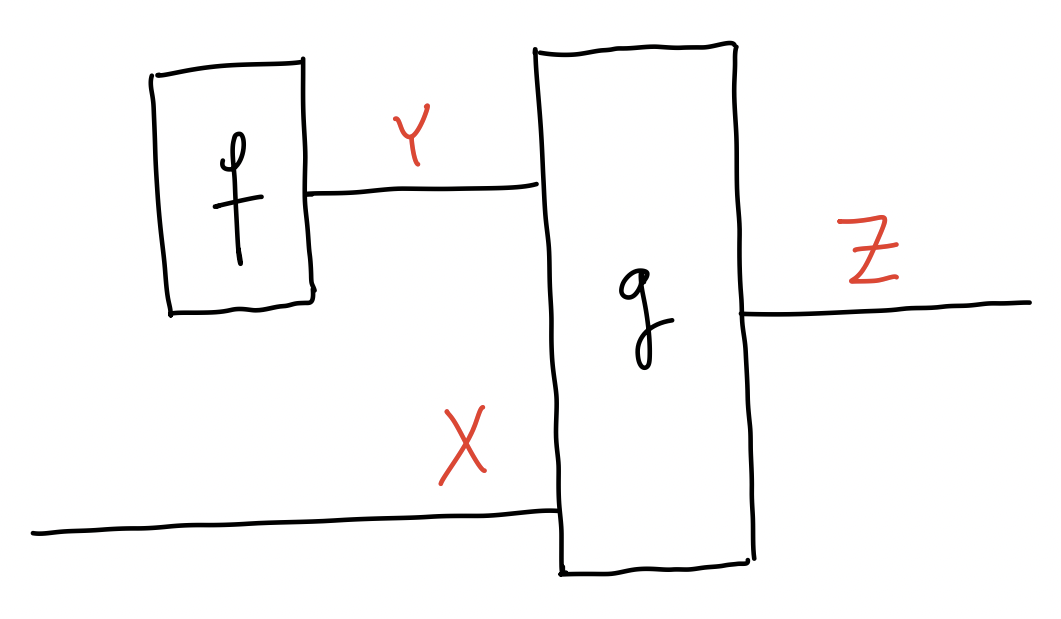
\includegraphics[width=0.5\linewidth]{pics/ExamStringDiagram1.png}
        \includesag{string_diag}
    \end{center}

    In each part of this exercise, we will specify a monoidal category and specific objects and morphisms to plug into the variables~$\Obja, \Objb, \Objc$ and~$\mora, \morb$ in this diagram.
    Your task is to compute the respective resulting morphism $\morc$ as dictated by the diagram.

    \begin{enumerate}
        \item In this part, let~$\tup{\CatC,\mtimescat,\idmoncat}$ be the monoidal category where~\CatC is the category~\Set of sets and functions,~$\mtimescat$ is the cartesian product of sets and functions, and~$\idmoncat$ is a chosen~$1$-element set that we denote by~$\singleton$.
              In the string diagram above, let~$\Obja = \wnumbers$,~$\Objb = \natnumbers$, and~$\Objc = \wnumbers$.
              Furthermore, let
              \begin{equation}
                  \mapa\colon \singleton \mto \Objb
              \end{equation}
              be the function with~$\mapa(\singletonel) = 5$, and let
              \begin{equation}
                  \defmapperiod{\mapb}{\natnumbers\cartprod \wnumbers}{\mto}{\wnumbers}{\tup{\elb,\ela}}{\elb+\ela}
              \end{equation}
              Compute the composite morphism $\morc$ described by the string diagram in this case.

        \item In this part, let~$\tup{\CatC,\mtimescat,\idmoncat}$ be the monoidal category where~\CatC is the category~\Rel of sets and relations,~$\mtimescat$ is the cartesian product of sets and relations, and~$\idmoncat$ is a chosen~$1$-element set that we again denote by~$\singleton$.
              In the string diagram, let~$\Obja = \wnumbers$,~$\Objb = \wnumbers$, and~$\Objc = \wnumbers$.
              Furthermore, let~$\mapa\colon \singleton \mto \wnumbers$ be the relation
              \begin{equation}
                  \mapa = \makeset{ \tup{\singletonel, \elb} \setin \singleton \cartprod \wnumbers \mid \elb \text{ is an even number}}
              \end{equation}
              and let~$\mapb \colon \wnumbers \cartprod \wnumbers \mto \wnumbers$ be the relation
              \begin{equation}
                  \mapb = \makeset{ \tup{\tup{\elb, \ela}, \elc} \setin (\wnumbers \cartprod \wnumbers) \cartprod \wnumbers \mid \elb = \ela = \elc}.
              \end{equation}

              Compute the composite morphism $\morc$ described by the string diagram in this case.

        \item In this part, let~$\tup{\CatC,\mtimescat,\idmoncat}$ be the monoidal category where~\CatC is the category of real vector spaces and real linear maps,~$\mtimescat$ is the direct sum, and~$\idmoncat$ is the~$0$-dimensional real vector space~$\makeset{0}$.
              In the string diagram, let~$\Obja = \Objb = \Objc = \reals^3$.
              Furthermore, let
              \begin{equation}
                  \mapa\colon \makeset{0} \mto \reals^3
              \end{equation}
              be the linear function with~$\mapa(0) = 0$, and let
              \begin{equation}
                  \defmapperiod{\mapb}{\reals^3\oplus \reals^3}{\mto}{\reals^3}{\tup{\elb,\ela}}{\elb+\ela}
              \end{equation}
              Compute the composite morphism $\morc$ described by the string diagram in this case.
    \end{enumerate}
\end{gradedexercise}
\solutionof{StringDiagrams}
